% Author: Marco Miani
\documentclass[varwidth=true, border=2pt]{standalone}

\usepackage{tikz}
\usetikzlibrary{positioning}
%% helper macros

% The 3D code is based on The drawing is based on Tomas M. Trzeciak's
% `Stereographic and cylindrical map projections example`:
% http://www.texample.net/tikz/examples/map-projections/
\newcommand\pgfmathsinandcos[3]{%
  \pgfmathsetmacro#1{sin(#3)}%
  \pgfmathsetmacro#2{cos(#3)}%
}
\newcommand\LongitudePlane[3][current plane]{%
  \pgfmathsinandcos\sinEl\cosEl{#2} % elevation
  \pgfmathsinandcos\sint\cost{#3} % azimuth
  \tikzset{#1/.estyle={cm={\cost,\sint*\sinEl,0,\cosEl,(0,0)}}}
}
\newcommand\LatitudePlane[3][current plane]{%
  \pgfmathsinandcos\sinEl\cosEl{#2} % elevation
  \pgfmathsinandcos\sint\cost{#3} % latitude
  \pgfmathsetmacro\yshift{\cosEl*\sint}
  \tikzset{#1/.estyle={cm={\cost,0,0,\cost*\sinEl,(0,\yshift)}}} %
}
\newcommand\DrawLongitudeCircle[2][1]{
  \LongitudePlane{\angEl}{#2}
  \tikzset{current plane/.prefix style={scale=#1}}
   % angle of "visibility"
  \pgfmathsetmacro\angVis{atan(sin(#2)*cos(\angEl)/sin(\angEl))} %
  \draw[current plane,thin,black] (\angVis:1) arc (\angVis:\angVis+180:1);
  \draw[current plane,thin,dashed] (\angVis-180:1) arc (\angVis-180:\angVis:1);
}%this is fake: for drawing the grid
\newcommand\DrawLongitudeCirclered[2][1]{
  \LongitudePlane{\angEl}{#2}
  \tikzset{current plane/.prefix style={scale=#1}}
   % angle of "visibility"
  \pgfmathsetmacro\angVis{atan(sin(#2)*cos(\angEl)/sin(\angEl))} %
  \draw[current plane,red,thick] (150:1) arc (150:180:1);
}%for drawing the grid
\newcommand\DLongredd[2][1]{
  \LongitudePlane{\angEl}{#2}
  \tikzset{current plane/.prefix style={scale=#1}}
   % angle of "visibility"
  \pgfmathsetmacro\angVis{atan(sin(#2)*cos(\angEl)/sin(\angEl))} %
  \draw[current plane,black,dashed, ultra thick] (150:1) arc (150:180:1);
}
\newcommand\DLatred[2][1]{
  \LatitudePlane{\angEl}{#2}
  \tikzset{current plane/.prefix style={scale=#1}}
  \pgfmathsetmacro\sinVis{sin(#2)/cos(#2)*sin(\angEl)/cos(\angEl)}
  % angle of "visibility"
  \pgfmathsetmacro\angVis{asin(min(1,max(\sinVis,-1)))}
  \draw[current plane,dashed,black,ultra thick] (-50:1) arc (-50:-35:1);

}
\newcommand\fillred[2][1]{
  \LongitudePlane{\angEl}{#2}
  \tikzset{current plane/.prefix style={scale=#1}}
   % angle of "visibility"
  \pgfmathsetmacro\angVis{atan(sin(#2)*cos(\angEl)/sin(\angEl))} %
  \draw[current plane,red,thin] (\angVis:1) arc (\angVis:\angVis+180:1);

}

\newcommand\DrawLatitudeCircle[2][1]{
  \LatitudePlane{\angEl}{#2}
  \tikzset{current plane/.prefix style={scale=#1}}
  \pgfmathsetmacro\sinVis{sin(#2)/cos(#2)*sin(\angEl)/cos(\angEl)}
  % angle of "visibility"
  \pgfmathsetmacro\angVis{asin(min(1,max(\sinVis,-1)))}
  \draw[current plane,thin,black] (\angVis:1) arc (\angVis:-\angVis-180:1);
  \draw[current plane,thin,dashed] (180-\angVis:1) arc (180-\angVis:\angVis:1);
}%Defining functions to draw limited latitude circles (for the red mesh)
\newcommand\DrawLatitudeCirclered[2][1]{
  \LatitudePlane{\angEl}{#2}
  \tikzset{current plane/.prefix style={scale=#1}}
  \pgfmathsetmacro\sinVis{sin(#2)/cos(#2)*sin(\angEl)/cos(\angEl)}
  % angle of "visibility"
  \pgfmathsetmacro\angVis{asin(min(1,max(\sinVis,-1)))}
  %\draw[current plane,red,thick] (-\angVis-50:1) arc (-\angVis-50:-\angVis-20:1);
\draw[current plane,red,thick] (-50:1) arc (-50:-35:1);

}

\tikzset{%
  >=latex,
  inner sep=0pt,%
  outer sep=2pt,%
  mark coordinate/.style={inner sep=0pt,outer sep=0pt,minimum size=3pt,
    fill=black,circle}%
}
\usepackage{amsmath}
\usetikzlibrary{arrows}
\pagestyle{empty}
\usepackage{pgfplots}
\usetikzlibrary{calc,fadings,decorations.pathreplacing}

\begin{document}
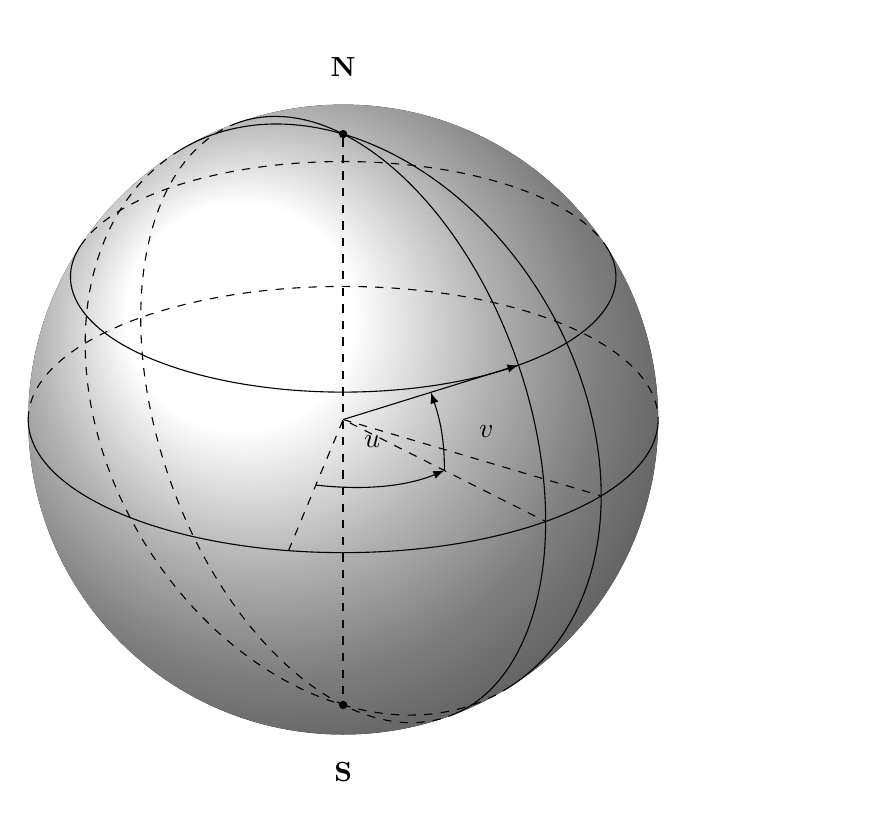
\begin{tikzpicture}[scale=1,every node/.style={minimum size=1cm}]
%% some definitions

\def\R{4} % sphere radius

\def\angEl{25} % elevation angle
\def\angAz{-100} % azimuth angle
\def\angPhiOne{-50} % longitude of point P
\def\angPhiTwo{-35} % longitude of point Q
\def\angBeta{30} % latitude of point P and Q

%% working planes

\pgfmathsetmacro\H{\R*cos(\angEl)} % distance to north pole
\LongitudePlane[xzplane]{\angEl}{\angAz}
\LongitudePlane[pzplane]{\angEl}{\angPhiOne}
\LongitudePlane[qzplane]{\angEl}{\angPhiTwo}
\LatitudePlane[equator]{\angEl}{0}
\fill[ball color=white!10] (0,0) circle (\R); % 3D lighting effect
\coordinate (O) at (0,0);
\coordinate[mark coordinate] (N) at (0,\H);
\coordinate[mark coordinate] (S) at (0,-\H);
\path[xzplane] (\R,0) coordinate (XE);

%defining points outsided the area bounded by the sphere
\path[qzplane] (\angBeta:\R+5.2376) coordinate (XEd);
\path[pzplane] (\angBeta:\R) coordinate (P);%fino alla sfera
\path[pzplane] (\angBeta:\R+5.2376) coordinate (Pd);%sfora di una quantità pari a 10 dopo la sfera
\path[pzplane] (\angBeta:\R+5.2376) coordinate (Td);%sfora di una quantità pari a 10 dopo la sfera
\path[pzplane] (\R,0) coordinate (PE);
\path[pzplane] (\R+4,0) coordinate (PEd);
\path[qzplane] (\angBeta:\R) coordinate (Q);
\path[qzplane] (\angBeta:\R) coordinate (Qd);%sfora di una quantità pari a 10 dopo la sfera

\path[qzplane] (\R,0) coordinate (QE);
\path[qzplane] (\R+4,0) coordinate (QEd);%sfora di una quantità 10 dalla sfera sul piano equat.


\DrawLongitudeCircle[\R]{\angPhiOne} % pzplane
\DrawLongitudeCircle[\R]{\angPhiTwo} % qzplane
\DrawLatitudeCircle[\R]{\angBeta}
\DrawLatitudeCircle[\R]{0} % equator
%labelling north and south
\node[above=8pt] at (N) {$\mathbf{N}$};
\node[below=8pt] at (S) {$\mathbf{S}$};

\draw[-,dashed, thick] (N) -- (S);
\draw[->] (O) -- (P);
\draw[dashed] (XE) -- (O) -- (PE);
\draw[dashed] (O) -- (QE);

\draw[pzplane,->,thin] (0:0.5*\R) to[bend right=15]
    node[midway,right] {$v$} (\angBeta:0.5*\R);
\path[pzplane] (0.5*\angBeta:\R) node[right] {$$};
\path[qzplane] (0.5*\angBeta:\R) node[right] {$$};
\draw[equator,->,thin] (\angAz:0.5*\R) to[bend right=30]
    node[pos=0.4,above] {$u$} (\angPhiOne:0.5*\R);

\end{tikzpicture}
\end{document}
